\section{Command-line testing}

You should review the advice in Section~\ref{sec:examples}, now that you've written some more substantial programs.
Remember, it's more effective to program and debug your code little by little than to attempt writing everything at once.
And once you've completed programming an algorithm, it's important to test that it works correctly on a variety of inputs.

Throughout the book, we will illustrate techniques for testing your programs.
Most if not all testing is based on a simple idea: does the program do what we expect it to do?
For simple programs, it's not difficult to run them several times and see what happens.
But at some point, you will get tired of typing the same test cases over and over.

We can automate the process of entering input and comparing {\em expected output} with {\em actual output} using the command line.
The basic idea is to store the test cases in plain text files and trick Java into thinking they are coming from the keyboard.
Here are step by step instructions.

\begin{enumerate}

\item Make sure you can compile and run the {\tt Convert.java} example in the previous section.
%You can also download a copy from \url{http://thinkjava.org/}.

\item In the same directory as {\tt Convert.java}, create a plain text file named {\tt test.in} (``in'' is for input).
Enter the following line and save the file.

\begin{stdout}
193.04
\end{stdout}

\item Create a second plain text file named {\tt test.exp} (``exp'' is for expected).
Enter the following line and save the file.

\begin{stdout}
193.04 cm = 6 ft, 4 in
\end{stdout}

\item Open a terminal, and change to the directory with these files.
Run the following command to test the program.

\begin{stdout}
java Convert < test.in > test.out
\end{stdout}

\end{enumerate}

\index{redirection operator}

On the command line, {\tt <} and {\tt >} are {\bf redirection operators}.
The first one redirects the contents of {\tt test.in} to \java{System.in}, as if it were entered from the keyboard.
The second one redirects the contents of \java{System.out} to a new file {\tt test.out}, much like a screen capture.
In other words, the {\tt test.out} file contains the output of your program.

% ABD: Since I killed the previous reference to abstraction, I am inclined
% to kill this one too.  The problem in both places is that it pulls the
% focus off topic.

%Redirecting a program's input and output is an example of how computer scientists use abstraction.
%Notice that \java{System.in} is not called \java{Keyboard}, and \java{System.out} is not called \java{Display}.
%In practice, these objects could be text files, network connections, microphones and speakers, or some other byte streams.
%What's great is that doesn't change anything about how you write the code.

By the way, it's perfectly okay to compile your programs in DrJava (or some other environment) and run them from the command line.
Knowing both techniques allows you to use the right tool for the job.

At this point, we just need to compare the contents {\tt test.out} with {\tt test.exp}.
If the files are the same, then the program outputted what we expected it to output.
If not, then we found a bug, and we can use the output to begin debugging our program.
Fortunately, there's a simple way to compare files on the command line:

\begin{stdout}
diff test.exp test.out
\end{stdout}

The {\tt diff} utility summarizes the differences between two files.
If there are no differences, then it prints nothing, which in our case is what we want.
If the expected output differs from the actual output, then we need to continue debugging.
Usually the program is at fault, and {\tt diff} provides some insight about what is broken.
But there's also a chance that we have a correct program and the expected output is wrong.

Interpreting the results from {\tt diff} can be confusing, but fortunately there are many graphical tools that show the differences between two files.
For example, on Windows you can install WinMerge, on Mac you can use {\tt opendiff} (which comes with Xcode), and on Linux there's {\tt meld}.
Regardless what tool you use, the goal is the same.
Debug your program until the actual output is {\it identical} to the expected output.

\begin{figure}[!h]
\begin{center}
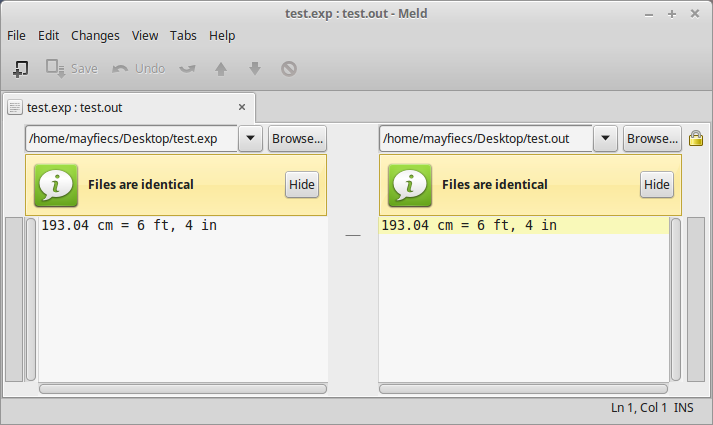
\includegraphics[width=0.9\textwidth]{figs/meld.png}
\caption{Using {\tt meld} to compare the expected output with the actual output.}
\end{center}
\end{figure}


\section{Tracing with a debugger}
\label{debugger}

\index{debugger}

Another way to visualize variables and parameters is to use a {\bf debugger}.
Most debuggers make it possible to:

\index{breakpoint}

\begin{enumerate}
\item Set a {\bf breakpoint}, which is line where you want the program to pause.
\item Step through the code one line at a time and watch what it does.
\item Check the values of variables and see when and how they change.
\end{enumerate}

%ABD: Do we want to move this to the web page?  It is specific to DrJava,
% and it's a little weird that we switch to the imperative here.

For example, open any program in DrJava and move the cursor to the first line of \java{main}.
Press Ctrl+B to toggle a breakpoint on the current line; it should now be highlighted in red.
Press Ctrl+Shift+D to turn on Debug Mode; a new pane should appear at the bottom of the window.
(These commands are also available from the {\em Debugger} menu, in case you forget the shortcut keys.)

\index{call stack}

When you run the program, execution pauses at the first breakpoint.
The debug pane shows the {\bf call stack}, with the current method on top of the stack.
You might be surprised to see how many methods were called before the \java{main} method!
To the right are several buttons that allow you to step through the code at your own pace.
You can also press ``Automatic Trace'' to watch DrJava run your code one line at a time.

\begin{figure}[!h]
\begin{center}
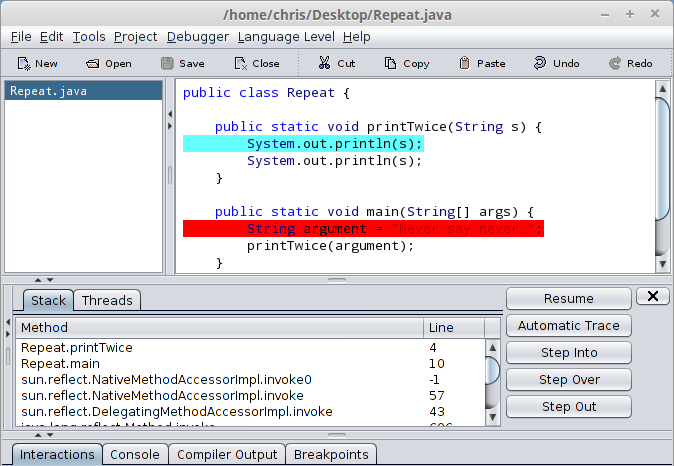
\includegraphics[width=\textwidth]{figs/debugger.png}
\caption{Screenshot of the DrJava debugger.
Execution is currently paused on the first line of \java{printTwice}.
There is a breakpoint on the first line of \java{main}.}
\end{center}
\end{figure}

Using a debugger is like having the computer proofread your code out loud.
When the program is paused, you can examine (or even change) the value of any variable using the Interactions Pane.
Tracing allows you to verify how control and data passes from one method to another.
%You can edit your code while debugging it, but the changes won't take effect until after you compile.
%The result can be confusing, so we don't recommend it.
%The debugger may get out of sync if you add or delete multiple lines of code while the program is paused.
You might expect the code do one thing, but then the debugger shows it doing something else.
At that moment, you gain insight about what may be wrong with the code.


\section{DrJava interactions}

A good way to gain experience with relational and logical operators is to use the Interactions Pane of DrJava.
As shown in Figure~\ref{fig:drjava}, you can declare several variables and {\it interactively} test your logic skills.
Don't forget that you can try out many of the examples in this book this same way.

% TODO: consider making this an exercise

\begin{figure}[!h]
\begin{center}
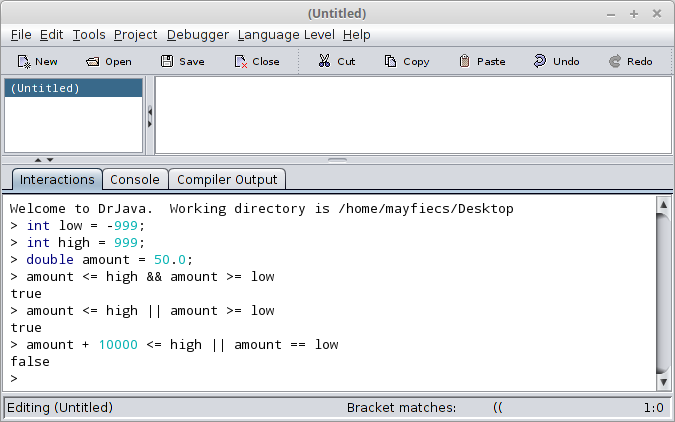
\includegraphics[width=\textwidth]{figs/drjava-logic.png}
\caption{Screenshot of the Interactions Pane in DrJava.}
\label{fig:drjava}
\end{center}
\end{figure}

There is one subtle detail to note when using the Interactions feature.
If you don't end an expression (or statement) with a semicolon, DrJava automatically prints its value.
Notice in Figure~\ref{fig:drjava} how the variable declarations end with semicolons, but the logic expressions in the following lines do not.

What's nice about this feature is that you don't have to create a new class, declare a main method, write arbitrary expressions inside \java{System.out.println} statements, save the source file, and get all of your code to compile in advance.
In addition, you can press the up/down arrows on the keyboard to repeat previous commands and experiment with incremental differences.

\index{order of operations}
\index{precedence}

Notice how none of the expressions in this example require parentheses.
Java evaluates arithmetic operators first, then the relational operators, then logical operators, and finally the assignment operator.
Do a web search for ``java operator precedence'' to see the complete list of rules.
If two operators have the same precedence, Java evaluates them from left to right.
